\begin{tikzpicture}
\pgfdeclareplotmark{cross} {
\pgfpathmoveto{\pgfpoint{-0.3\pgfplotmarksize}{\pgfplotmarksize}}
\pgfpathlineto{\pgfpoint{+0.3\pgfplotmarksize}{\pgfplotmarksize}}
\pgfpathlineto{\pgfpoint{+0.3\pgfplotmarksize}{0.3\pgfplotmarksize}}
\pgfpathlineto{\pgfpoint{+1\pgfplotmarksize}{0.3\pgfplotmarksize}}
\pgfpathlineto{\pgfpoint{+1\pgfplotmarksize}{-0.3\pgfplotmarksize}}
\pgfpathlineto{\pgfpoint{+0.3\pgfplotmarksize}{-0.3\pgfplotmarksize}}
\pgfpathlineto{\pgfpoint{+0.3\pgfplotmarksize}{-1.\pgfplotmarksize}}
\pgfpathlineto{\pgfpoint{-0.3\pgfplotmarksize}{-1.\pgfplotmarksize}}
\pgfpathlineto{\pgfpoint{-0.3\pgfplotmarksize}{-0.3\pgfplotmarksize}}
\pgfpathlineto{\pgfpoint{-1.\pgfplotmarksize}{-0.3\pgfplotmarksize}}
\pgfpathlineto{\pgfpoint{-1.\pgfplotmarksize}{0.3\pgfplotmarksize}}
\pgfpathlineto{\pgfpoint{-0.3\pgfplotmarksize}{0.3\pgfplotmarksize}}
\pgfpathclose
\pgfusepathqstroke
}
\pgfdeclareplotmark{cross*} {
\pgfpathmoveto{\pgfpoint{-0.3\pgfplotmarksize}{\pgfplotmarksize}}
\pgfpathlineto{\pgfpoint{+0.3\pgfplotmarksize}{\pgfplotmarksize}}
\pgfpathlineto{\pgfpoint{+0.3\pgfplotmarksize}{0.3\pgfplotmarksize}}
\pgfpathlineto{\pgfpoint{+1\pgfplotmarksize}{0.3\pgfplotmarksize}}
\pgfpathlineto{\pgfpoint{+1\pgfplotmarksize}{-0.3\pgfplotmarksize}}
\pgfpathlineto{\pgfpoint{+0.3\pgfplotmarksize}{-0.3\pgfplotmarksize}}
\pgfpathlineto{\pgfpoint{+0.3\pgfplotmarksize}{-1.\pgfplotmarksize}}
\pgfpathlineto{\pgfpoint{-0.3\pgfplotmarksize}{-1.\pgfplotmarksize}}
\pgfpathlineto{\pgfpoint{-0.3\pgfplotmarksize}{-0.3\pgfplotmarksize}}
\pgfpathlineto{\pgfpoint{-1.\pgfplotmarksize}{-0.3\pgfplotmarksize}}
\pgfpathlineto{\pgfpoint{-1.\pgfplotmarksize}{0.3\pgfplotmarksize}}
\pgfpathlineto{\pgfpoint{-0.3\pgfplotmarksize}{0.3\pgfplotmarksize}}
\pgfpathclose
\pgfusepathqfillstroke
}
\pgfdeclareplotmark{newstar} {
\pgfpathmoveto{\pgfqpoint{0pt}{\pgfplotmarksize}}
\pgfpathlineto{\pgfqpointpolar{44}{0.5\pgfplotmarksize}}
\pgfpathlineto{\pgfqpointpolar{18}{\pgfplotmarksize}}
\pgfpathlineto{\pgfqpointpolar{-20}{0.5\pgfplotmarksize}}
\pgfpathlineto{\pgfqpointpolar{-54}{\pgfplotmarksize}}
\pgfpathlineto{\pgfqpointpolar{-90}{0.5\pgfplotmarksize}}
\pgfpathlineto{\pgfqpointpolar{234}{\pgfplotmarksize}}
\pgfpathlineto{\pgfqpointpolar{198}{0.5\pgfplotmarksize}}
\pgfpathlineto{\pgfqpointpolar{162}{\pgfplotmarksize}}
\pgfpathlineto{\pgfqpointpolar{134}{0.5\pgfplotmarksize}}
\pgfpathclose
\pgfusepathqstroke
}
\pgfdeclareplotmark{newstar*} {
\pgfpathmoveto{\pgfqpoint{0pt}{\pgfplotmarksize}}
\pgfpathlineto{\pgfqpointpolar{44}{0.5\pgfplotmarksize}}
\pgfpathlineto{\pgfqpointpolar{18}{\pgfplotmarksize}}
\pgfpathlineto{\pgfqpointpolar{-20}{0.5\pgfplotmarksize}}
\pgfpathlineto{\pgfqpointpolar{-54}{\pgfplotmarksize}}
\pgfpathlineto{\pgfqpointpolar{-90}{0.5\pgfplotmarksize}}
\pgfpathlineto{\pgfqpointpolar{234}{\pgfplotmarksize}}
\pgfpathlineto{\pgfqpointpolar{198}{0.5\pgfplotmarksize}}
\pgfpathlineto{\pgfqpointpolar{162}{\pgfplotmarksize}}
\pgfpathlineto{\pgfqpointpolar{134}{0.5\pgfplotmarksize}}
\pgfpathclose
\pgfusepathqfillstroke
}
\definecolor{c}{rgb}{1,1,1};
\draw [color=c, fill=c] (0,0) rectangle (20,10.2253);
\draw [color=c, fill=c] (2,1.02253) rectangle (18,9.2028);
\definecolor{c}{rgb}{0,0,0};
\draw [c,line width=0.9] (2,1.02253) -- (2,9.2028) -- (18,9.2028) -- (18,1.02253) -- (2,1.02253);
\definecolor{c}{rgb}{1,1,1};
\draw [color=c, fill=c] (2,1.02253) rectangle (18,9.2028);
\definecolor{c}{rgb}{0,0,0};
\draw [c,line width=0.9] (2,1.02253) -- (2,9.2028) -- (18,9.2028) -- (18,1.02253) -- (2,1.02253);
\definecolor{c}{rgb}{0.977,0.977044,0.0583656};
\draw [color=c, fill=c] (2,1.02253) rectangle (5.37553,2.55633);
\definecolor{c}{rgb}{0.884975,0.752825,0.292488};
\draw [color=c, fill=c] (5.37553,1.02253) rectangle (8.75105,2.55633);
\definecolor{c}{rgb}{0.453559,0.742331,0.504766};
\draw [color=c, fill=c] (8.75105,1.02253) rectangle (11.2489,2.55633);
\definecolor{c}{rgb}{0.322347,0.730556,0.570878};
\draw [color=c, fill=c] (12.2616,1.02253) rectangle (15.5021,2.55633);
\definecolor{c}{rgb}{0.453559,0.742331,0.504766};
\draw [color=c, fill=c] (15.5021,1.02253) rectangle (18,2.55633);
\definecolor{c}{rgb}{0.701397,0.739462,0.397147};
\draw [color=c, fill=c] (2,2.55633) rectangle (5.37553,3.57887);
\definecolor{c}{rgb}{0.453559,0.742331,0.504766};
\draw [color=c, fill=c] (5.37553,2.55633) rectangle (8.75105,3.57887);
\definecolor{c}{rgb}{0.1802,0.7178,0.6425};
\draw [color=c, fill=c] (8.75105,2.55633) rectangle (11.2489,3.57887);
\draw [color=c, fill=c] (12.2616,2.55633) rectangle (15.5021,3.57887);
\definecolor{c}{rgb}{0.322347,0.730556,0.570878};
\draw [color=c, fill=c] (15.5021,2.55633) rectangle (18,3.57887);
\definecolor{c}{rgb}{0.701397,0.739462,0.397147};
\draw [color=c, fill=c] (2,3.57887) rectangle (5.37553,5.11267);
\definecolor{c}{rgb}{0.322347,0.730556,0.570878};
\draw [color=c, fill=c] (5.37553,3.57887) rectangle (8.75105,5.11267);
\definecolor{c}{rgb}{0.116419,0.686966,0.702991};
\draw [color=c, fill=c] (8.75105,3.57887) rectangle (11.2489,5.11267);
\definecolor{c}{rgb}{0.1802,0.7178,0.6425};
\draw [color=c, fill=c] (12.2616,3.57887) rectangle (15.5021,5.11267);
\draw [color=c, fill=c] (15.5021,3.57887) rectangle (18,5.11267);
\definecolor{c}{rgb}{0.453559,0.742331,0.504766};
\draw [color=c, fill=c] (2,5.11267) rectangle (5.37553,9.2028);
\definecolor{c}{rgb}{0.116419,0.686966,0.702991};
\draw [color=c, fill=c] (5.37553,5.11267) rectangle (8.75105,9.2028);
\draw [color=c, fill=c] (8.75105,5.11267) rectangle (11.2489,9.2028);
\draw [color=c, fill=c] (12.2616,5.11267) rectangle (15.5021,9.2028);
\definecolor{c}{rgb}{0.1802,0.7178,0.6425};
\draw [color=c, fill=c] (15.5021,5.11267) rectangle (18,9.2028);
\definecolor{c}{rgb}{0,0,0};
\draw (3.68776,1.78943) node[scale=1.448681, color=c, rotate=1]{$\genfrac{}{}{0pt}{}{2.00874}{\pm 0.032851}$};
\draw (7.06329,1.78943) node[scale=0.448681, color=c, rotate=1]{$\genfrac{}{}{0pt}{}{1.5119}{\pm 0.0414325}$};
\draw (10,1.78943) node[scale=0.448681, color=c, rotate=1]{$\genfrac{}{}{0pt}{}{1.20253}{\pm 0.0185689}$};
\draw (13.8819,1.78943) node[scale=0.448681, color=c, rotate=1]{$\genfrac{}{}{0pt}{}{1.02046}{\pm 0.0118223}$};
\draw (16.7511,1.78943) node[scale=0.448681, color=c, rotate=1]{$\genfrac{}{}{0pt}{}{1.1153}{\pm 0.0129772}$};
\draw (3.68776,3.0676) node[scale=0.448681, color=c, rotate=1]{$\genfrac{}{}{0pt}{}{1.39202}{\pm 0.0146212}$};
\draw (7.06329,3.0676) node[scale=0.448681, color=c, rotate=1]{$\genfrac{}{}{0pt}{}{1.16483}{\pm 0.0115263}$};
\draw (10,3.0676) node[scale=0.448681, color=c, rotate=1]{$\genfrac{}{}{0pt}{}{0.972198}{\pm 0.0096481}$};
\draw (13.8819,3.0676) node[scale=0.448681, color=c, rotate=1]{$\genfrac{}{}{0pt}{}{0.963159}{\pm 0.00771131}$};
\draw (16.7511,3.0676) node[scale=0.448681, color=c, rotate=1]{$\genfrac{}{}{0pt}{}{1.01539}{\pm 0.00852304}$};
\draw (3.68776,4.34577) node[scale=0.448681, color=c, rotate=1]{$\genfrac{}{}{0pt}{}{1.35402}{\pm 0.0212578}$};
\draw (7.06329,4.34577) node[scale=0.448681, color=c, rotate=1]{$\genfrac{}{}{0pt}{}{1.02707}{\pm 0.0160391}$};
\draw (10,4.34577) node[scale=0.448681, color=c, rotate=1]{$\genfrac{}{}{0pt}{}{0.900305}{\pm 0.0136784}$};
\draw (13.8819,4.34577) node[scale=0.448681, color=c, rotate=1]{$\genfrac{}{}{0pt}{}{0.939213}{\pm 0.0110738}$};
\draw (16.7511,4.34577) node[scale=0.448681, color=c, rotate=1]{$\genfrac{}{}{0pt}{}{0.951099}{\pm 0.013204}$};
\draw (3.68776,7.15773) node[scale=0.448681, color=c, rotate=1]{$\genfrac{}{}{0pt}{}{1.17035}{\pm 0.126888}$};
\draw (7.06329,7.15773) node[scale=0.448681, color=c, rotate=1]{$\genfrac{}{}{0pt}{}{0.880072}{\pm 0.0515612}$};
\draw (10,7.15773) node[scale=0.448681, color=c, rotate=1]{$\genfrac{}{}{0pt}{}{0.888044}{\pm 0.0561041}$};
\draw (13.8819,7.15773) node[scale=0.448681, color=c, rotate=1]{$\genfrac{}{}{0pt}{}{0.900557}{\pm 0.0434463}$};
\draw (16.7511,7.15773) node[scale=0.448681, color=c, rotate=1]{$\genfrac{}{}{0pt}{}{0.977716}{\pm 0.0474501}$};
\draw [c,line width=0.9] (2,1.02253) -- (18,1.02253);
\draw [anchor=north] (3.68776,0.899829) node[scale=0.517709, color=c, rotate=0]{[0.0 - 0.5]};
\draw [anchor=north] (7.06329,0.899829) node[scale=0.517709, color=c, rotate=0]{[0.5 - 1.0]};
\draw [anchor=north] (10,0.899829) node[scale=0.517709, color=c, rotate=0]{[1.0 - 1.37]};
\draw [anchor=north] (11.7553,0.899829) node[scale=0.517709, color=c, rotate=0]{[1.37 - 1.52]};
\draw [anchor=north] (13.8819,0.899829) node[scale=0.517709, color=c, rotate=0]{[1.52 - 2.0]};
\draw [anchor=north] (16.7511,0.899829) node[scale=0.517709, color=c, rotate=0]{[2.0 - 2.37]};
\draw [c,line width=0.9] (2,1.26794) -- (2,1.02253);
\draw [c,line width=0.9] (5.37553,1.26794) -- (5.37553,1.02253);
\draw [c,line width=0.9] (8.75105,1.26794) -- (8.75105,1.02253);
\draw [c,line width=0.9] (12.1266,1.26794) -- (12.1266,1.02253);
\draw [c,line width=0.9] (15.5021,1.26794) -- (15.5021,1.02253);
\draw [c,line width=0.9] (15.5021,1.26794) -- (15.5021,1.02253);
\draw [anchor= east] (18,0.449915) node[scale=0.79382, color=c, rotate=0]{|eta|};
\draw [c,line width=0.9] (2,1.02253) -- (2,9.2028);
\draw [anchor= east] (1.76,1.78943) node[scale=0.517709, color=c, rotate=0]{[20 - 35] };
\draw [anchor= east] (1.76,3.0676) node[scale=0.517709, color=c, rotate=0]{[35 - 45] };
\draw [anchor= east] (1.76,4.34577) node[scale=0.517709, color=c, rotate=0]{[45 - 60] };
\draw [anchor= east] (1.76,7.15773) node[scale=0.517709, color=c, rotate=0]{[60 - 100]};
\draw [c,line width=0.9] (2.48,1.02253) -- (2,1.02253);
\draw [c,line width=0.9] (2.48,3.0676) -- (2,3.0676);
\draw [c,line width=0.9] (2.48,5.11267) -- (2,5.11267);
\draw [c,line width=0.9] (2.48,7.15773) -- (2,7.15773);
\draw [c,line width=0.9] (2.48,9.2028) -- (2,9.2028);
\draw [anchor= east] (0.383139,9.2028) node[scale=0.79382, color=c, rotate=90]{pT [GeV]};
\definecolor{c}{rgb}{0.150523,0.241303,0.660565};
\draw [color=c, fill=c] (18.1,1.02253) rectangle (19,1.43155);
\definecolor{c}{rgb}{0.0880387,0.322448,0.802768};
\draw [color=c, fill=c] (18.1,1.43155) rectangle (19,1.84056);
\definecolor{c}{rgb}{0.0633125,0.391444,0.861859};
\draw [color=c, fill=c] (18.1,1.84056) rectangle (19,2.24957);
\definecolor{c}{rgb}{0.0703625,0.445519,0.850647};
\draw [color=c, fill=c] (18.1,2.24957) rectangle (19,2.65859);
\definecolor{c}{rgb}{0.078,0.5041,0.8385};
\draw [color=c, fill=c] (18.1,2.65859) rectangle (19,3.0676);
\definecolor{c}{rgb}{0.0557375,0.560081,0.819366};
\draw [color=c, fill=c] (18.1,3.0676) rectangle (19,3.47661);
\definecolor{c}{rgb}{0.033475,0.616063,0.800231};
\draw [color=c, fill=c] (18.1,3.47661) rectangle (19,3.88563);
\definecolor{c}{rgb}{0.0526375,0.656131,0.763481};
\draw [color=c, fill=c] (18.1,3.88563) rectangle (19,4.29464);
\definecolor{c}{rgb}{0.116419,0.686966,0.702991};
\draw [color=c, fill=c] (18.1,4.29464) rectangle (19,4.70365);
\definecolor{c}{rgb}{0.1802,0.7178,0.6425};
\draw [color=c, fill=c] (18.1,4.70365) rectangle (19,5.11267);
\definecolor{c}{rgb}{0.322347,0.730556,0.570878};
\draw [color=c, fill=c] (18.1,5.11267) rectangle (19,5.52168);
\definecolor{c}{rgb}{0.453559,0.742331,0.504766};
\draw [color=c, fill=c] (18.1,5.52168) rectangle (19,5.93069);
\definecolor{c}{rgb}{0.584194,0.746125,0.444394};
\draw [color=c, fill=c] (18.1,5.93069) rectangle (19,6.3397);
\definecolor{c}{rgb}{0.701397,0.739462,0.397147};
\draw [color=c, fill=c] (18.1,6.3397) rectangle (19,6.74872);
\definecolor{c}{rgb}{0.8186,0.7328,0.3499};
\draw [color=c, fill=c] (18.1,6.74872) rectangle (19,7.15773);
\definecolor{c}{rgb}{0.884975,0.752825,0.292488};
\draw [color=c, fill=c] (18.1,7.15773) rectangle (19,7.56674);
\definecolor{c}{rgb}{0.956881,0.774519,0.230291};
\draw [color=c, fill=c] (18.1,7.56674) rectangle (19,7.97576);
\definecolor{c}{rgb}{0.992,0.823138,0.170006};
\draw [color=c, fill=c] (18.1,7.97576) rectangle (19,8.38477);
\definecolor{c}{rgb}{0.9842,0.903169,0.111953};
\draw [color=c, fill=c] (18.1,8.38477) rectangle (19,8.79378);
\definecolor{c}{rgb}{0.977,0.977044,0.0583656};
\draw [color=c, fill=c] (18.1,8.79378) rectangle (19,9.2028);
\definecolor{c}{rgb}{0,0,0};
\draw [c,line width=0.9] (19,1.02253) -- (19,9.2028);
\draw [c,line width=0.9] (18.52,1.02253) -- (19,1.02253);
\draw [c,line width=0.9] (18.52,1.837) -- (19,1.837);
\draw [c,line width=0.9] (18.52,2.65147) -- (19,2.65147);
\draw [c,line width=0.9] (18.52,3.46593) -- (19,3.46593);
\draw [c,line width=0.9] (18.52,4.2804) -- (19,4.2804);
\draw [c,line width=0.9] (18.52,5.09486) -- (19,5.09486);
\draw [c,line width=0.9] (18.52,5.90933) -- (19,5.90933);
\draw [c,line width=0.9] (18.52,6.7238) -- (19,6.7238);
\draw [c,line width=0.9] (18.52,7.53826) -- (19,7.53826);
\draw [c,line width=0.9] (18.52,8.35273) -- (19,8.35273);
\draw [c,line width=0.9] (18.52,9.1672) -- (19,9.1672);
\draw [c,line width=0.9] (18.52,9.1672) -- (19,9.1672);
\draw [anchor= west] (19.1,1.02253) node[scale=0.79382, color=c, rotate=0]{0};
\draw [anchor= west] (19.1,1.837) node[scale=0.79382, color=c, rotate=0]{0.2};
\draw [anchor= west] (19.1,2.65147) node[scale=0.79382, color=c, rotate=0]{0.4};
\draw [anchor= west] (19.1,3.46593) node[scale=0.79382, color=c, rotate=0]{0.6};
\draw [anchor= west] (19.1,4.2804) node[scale=0.79382, color=c, rotate=0]{0.8};
\draw [anchor= west] (19.1,5.09486) node[scale=0.79382, color=c, rotate=0]{1};
\draw [anchor= west] (19.1,5.90933) node[scale=0.79382, color=c, rotate=0]{1.2};
\draw [anchor= west] (19.1,6.7238) node[scale=0.79382, color=c, rotate=0]{1.4};
\draw [anchor= west] (19.1,7.53826) node[scale=0.79382, color=c, rotate=0]{1.6};
\draw [anchor= west] (19.1,8.35273) node[scale=0.79382, color=c, rotate=0]{1.8};
\draw [anchor= west] (19.1,9.1672) node[scale=0.79382, color=c, rotate=0]{2};
%\draw (10,9.89301) node[scale=1.06993, color=c, rotate=0]{2D fake rate scale factors};
\end{tikzpicture}
